% Section: Experiments
\section{Experiments} \label{sec:experiment}

\subsection{First Experiment}
Our first experiment is conducted on a one-dimensional data as shown in Figure~\ref{fig:data1}. In this experiment, we have a 543-point training set ranging from $x = -32$ to $x = 14$, and we want to predict some 67-point test set ranging from $x = 14$ to $x = 21$.


\begin{figure}[htp]
\begin{minipage}[htp]{1\linewidth}
	\centering
  	\subfloat{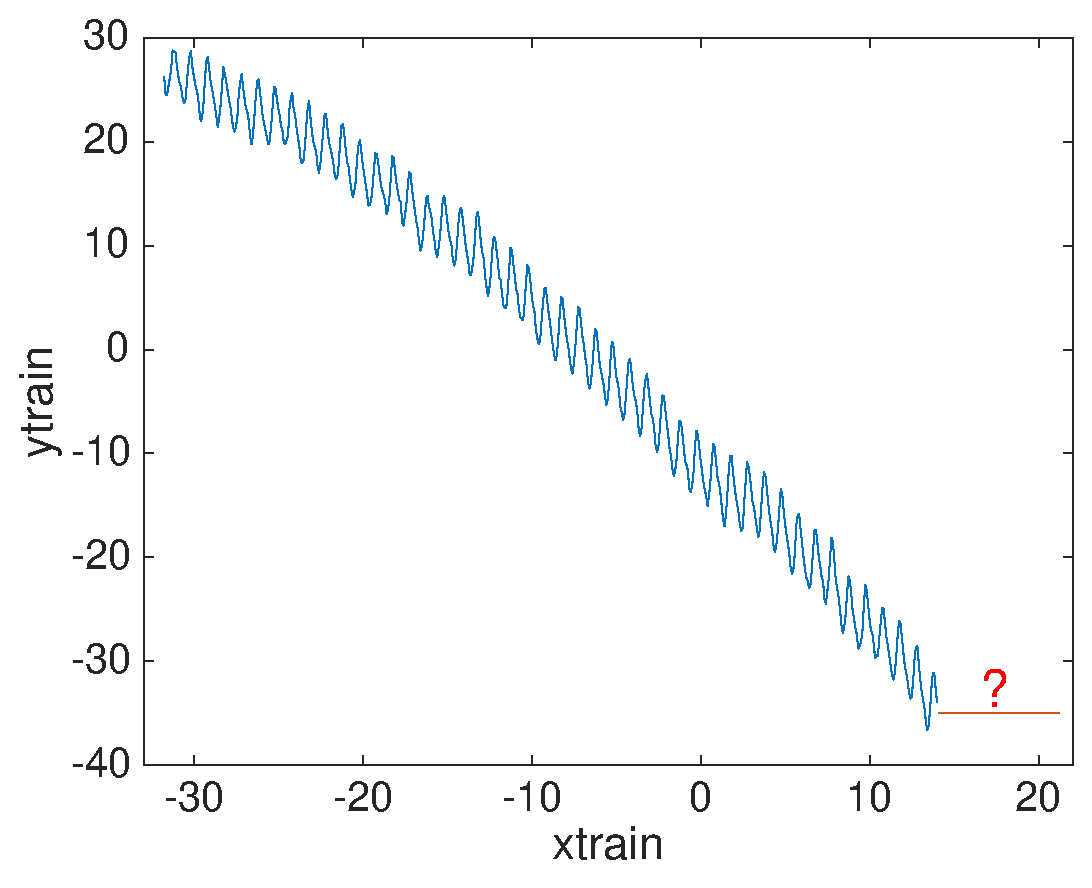
\includegraphics[width=0.7\textwidth]{figure/data1.eps}}
% \vspace{-0.1in}
\caption{A one-dimensional dataset}
\label{fig:data1} % FIG1
\end{minipage}
\vspace{-0.05in}
\end{figure}






\subsection{Second Experiment}

\begin{figure}[htp]
\begin{minipage}[htp]{1\linewidth}
	\centering
  	\subfloat{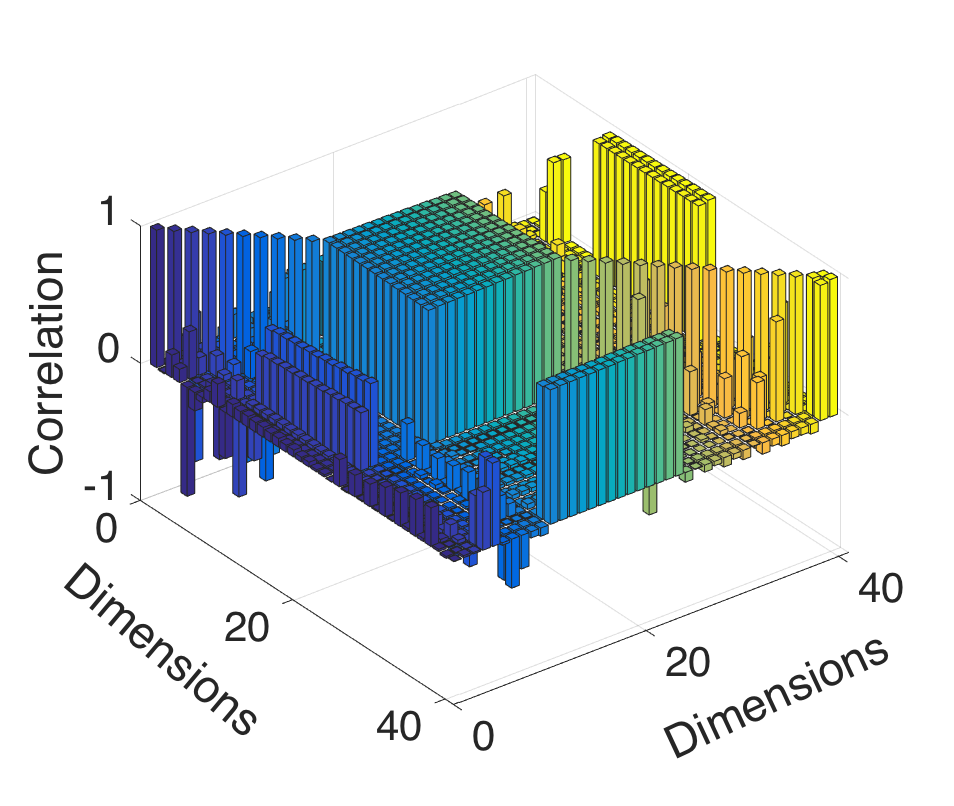
\includegraphics[width=0.9\textwidth]{figure/data2.eps}}
% \vspace{-0.1in}
\caption{A 40-dimensional dataset}
\label{fig:data1} % FIG1
\end{minipage}
\vspace{-0.05in}
\end{figure}






